\chapter{Other malware}

\section{Hajime}

Hajime was first discovered in October 2016 by security researchers at Rapidity Networks and it was given a Japanese name (meaning "beginning") thanks to its closed resemblance to Mirai. It mainly targets and infects IoT devices, exploiting default credentials and unpatched vulnerabilities. Once a device is infected, Hajime propagates itself by scanning the network and brute forcing credentials to gain access to the other devices. Unlike Mirai, Hajime has a decentralized P2P architecture, using a modified version of the BitTorrent protocol for communication. Another important difference is that, as of now, Hajime does not deliver any malicious payload and it seems that it secures the devices it infects, specifically, it blocks ports 23, 7547, 5555, and 5358, which are commonly used by other malware to infect devices, effectively preventing infection from others. There are different speculations related to the motivations behind Hajime, some say that it could be a vigilante malware, designed to protect IoT devices, or it could be a future threat.

\section{Goldoon}

\section{BotenaGo}

Identified in November 2021 by AT\&T Alien Labs researchers, BotenaGo is a backdoor that provides cybercriminals access to devices through 33 exploit functions. Their first analysis was performed by reverse engineering the malware's binary and it revealed that the malware associates each exploit function with a string that represents a potential target system, similar to a signature. This is needed because the malware sends a ``GET'' request to the target and then searches into the returned data for the signature. For example the string ``\texttt{Server: Boa/0.93.15}'' is mapped to the function \texttt{main\_infectFunctionGponFiber} which exploit the CVE-2020-8958 vulnerability. They also privide a search result on Shodan that shows 2 milion potential targets. This number decreased in the years as you can see in \Cref{fig:boa-shodan}. All the exploits can be found in \Cref{fig:all-vulnerabilities-botenago} which illustrates the \texttt{scannerInitExploit} from its source code.

\begin{figure}[ht]
    \centering
    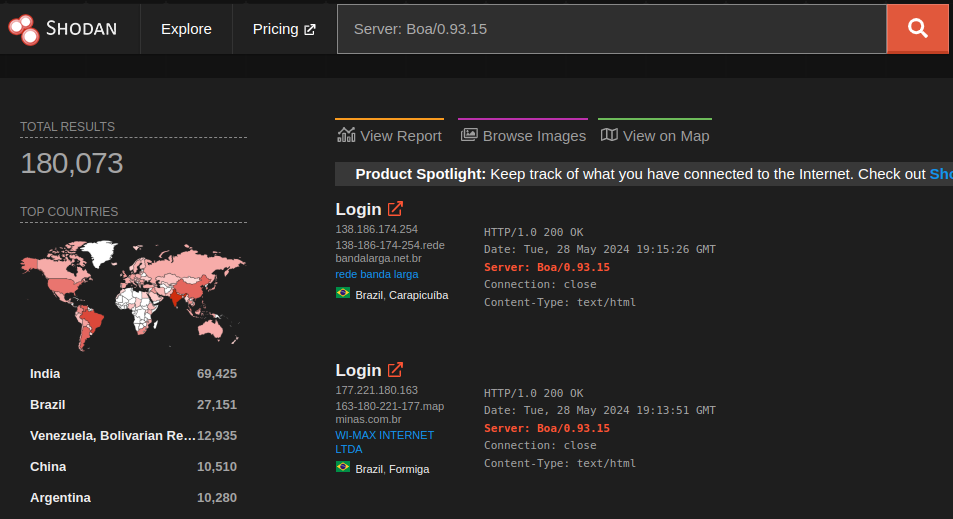
\includegraphics[scale=0.4]{resources/images/boa-shodan.png}
    \caption{Shodan search result for Boa/0.93.15}
    \label{fig:boa-shodan}
\end{figure}

The CNC has two ways of sending command to the infected device:

\begin{enumerate}
    \item Use one of the two backdoor ports (31412 and 19412) to send a command to the device. On port 19412, it lissens for the victim IP address and once received it tries each exploit on that IP.
    \item It listens on a system IO user input. For example it can be accessed locally by using telnet. 
\end{enumerate}

In 2022 its source code was leaked on GitHub and AT\&T Alien Labs provided another analysis which did not provide new information but confirmed the previous analysis. \cite{att-botenago-reverse,att-botenago-sourcecode}

\begin{figure}[ht]
    \centering
    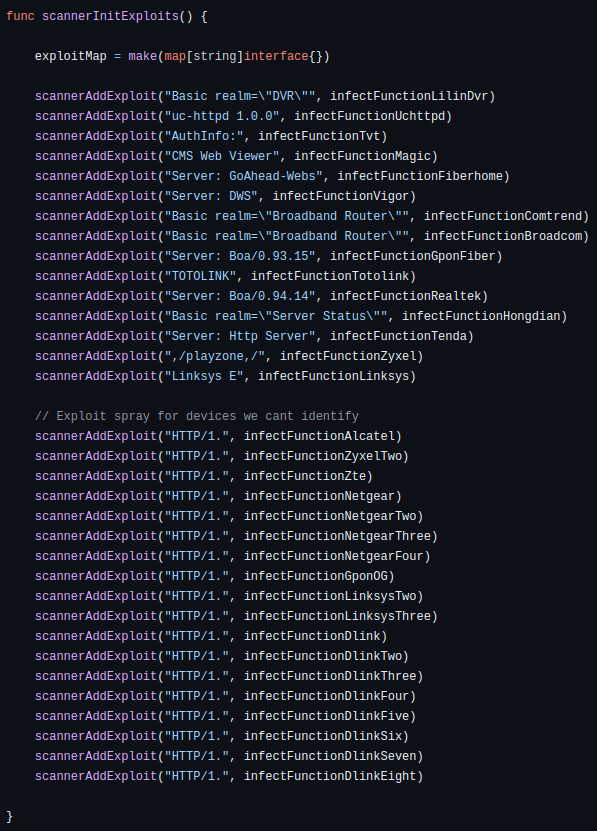
\includegraphics[scale=0.5]{resources/images/all-vulnerabilities-botenago.png}
    \caption{All the vulnerabilities exploited by BotenaGo}
    \label{fig:all-vulnerabilities-botenago}
\end{figure}

\section{Malware comparison}

\begin{table}
	\centering
	\begin{tabular}{|c|c|c|c|c|}
		\hline
		 & \textbf{Mirai} & \textbf{Hajime} & \textbf{Goldoon} & \textbf{BotenaGo} \\
		\hline
		\textbf{Spread} & Real-time-load & Brute force & Download source & Vulnerabilities exploitation \\
		\hline
		\textbf{Persistent} & No & No & Yes & Yes \\
		\hline
		\textbf{Code} & Open Source & Reversed & Reversed & Open Source \\
		\hline
		\textbf{Status} & Active (many variants) & Dormant? & Active & Active \\
		\hline
		\textbf{Control} & Only DDoS & No attacks & RCE and DDoS & RCE and DDOS \\
		\hline
	\end{tabular}
	\caption{Characteristics of Different Malware}
	\label{tab:malware_characteristics}
\end{table}

